\documentclass[12pt, reqno]{amsart}

\usepackage[
a4paper,% other options: a3paper, a5paper, etc
margin = 2.5cm
% use vmargin=2cm to make vertical margins equal to 2cm.
% us  hmargin=3cm to make horizontal margins equal to 3cm.
% use margin=3cm to make all margins  equal to 3cm.
]
{geometry}

\usepackage{amsmath}
\usepackage{amsfonts}
\usepackage{amsthm}
\usepackage{amssymb}
\usepackage{graphicx}
% \usepackage{ulem}

\title{Modelling Disease Spread}
\author{(Group 10) Subhodh Kotekal, Dongil Lee, Hongyang Li, Boyuan Yu}
\date{December 9, 2020}

\begin{document}
    \maketitle

    \section{Abstract}
    In this paper, we first review the standard SIR (Susceptible-Infected-Removed) model that simulate how disease spreads in a population, in which models of both discrete agent-based scheme and continuous ODE settings are discussed. In accordance with the pattern of physical interactions in reality, we then introduce the spatial component to the models so that infection rate is governed by the interaction radius in agent-based model and diffusion weight in the continuous model. In addition, we consider several variations on the SIR model that may better depicts the real world settings, including the steady state infection in continuous model, the effects of "lockdown" in discrete setting, the impact of vaccines and concatenated model in which parameters depend on current state. From various findings we had in our models, we conclude that strict travel restrictions typically have significant advantages on keeping infection level low, while such effective policies are better to be enacted promptly and remain effective in order to further cap down the infected population.
    \section{Introduction to the SIR model} \label{section:intro}

    The Susceptible-Infected-Removed Model for Disease Spread, which we will call the SIR model in the following discussion, is a model that puts each individual in the population into exactly one of three catagories: the \(S\) category consists of individuals susceptible to the disease, the \(I\) category consists of infected individuals, and the \(R\) category consists of individuals who have recovered from the illness and can no longer contract the disease. The parameter \(b\) controls the number infected per day after interacting with an infected individual, and \(k\) controls the number of recoveries per day. Together, we can formulate this model into a system of ordinary differential equations (see Appendix \ref{appendix:sir_ode_figs}). A discrete version of this model can be formulated consisting of \(N\) discrete individuals who interact with \(b\) random other individuals at each time step and \(k\) infected individuals recover at each time step. The ODE model stated above is, in a sense, the continuous limit of this discrete model.

    As stated, the SIR model posits that any individual interacts with all other individuals uniformly. This is not a realistic assumption as people in the real world usually only interact with spatially nearby individuals. In a continuous setting, a mathematically convenient path forward is to posit that movement of people is a diffusion in a two-dimensional plane, and we obtain a system of partial differential equations (see Appendix \ref{appendix:sir_pde}). The parameters \(b, k\) retain their interpretation from the original SIR model. The parameter \(p > 0\) is the diffusion weight and dictates the speed of diffusion. A discrete version of this model can be constructed in which individuals move in a two dimensional grid according to a symmetric random walk with step size \(p\). Each individual interacts with all other individuals within radius \(q\), and \(k\) infected individuals recover at each time step. Under a certain identification of parameters, the above PDE is the continuous limit of this discrete model. 

    \section{SIR Model} \label{section:SIR_model}

    \subsection{ODE model}
    To get a first sense of how the ODE version of the SIR model behaves, we started with a simple simulation. We considered the parameter configuration of \(k = 0.05, b = 10\) and \(i_0 = 0.0001\). In words, about \(5\%\) of those infected recover per day, there are about \(10\) interactions per day per individual that could spread the disease, the population size is \(10000\) individuals, and \(0.01\%\) of the population is infected at time \(0\). Simulating, we obtain Figure \ref{fig:simulation0} (all figures referenced in this section are found in Appendix \ref{appendix:sir_ode_figs}). The mirroring dynamics of the infected and recovered individuals agrees with intuition. 
    
    To examine how social distancing might affect the dynamics, we set \(b = 1\). We immediately notice that the time it takes for \(S(t)\) to drop to zero is about ten times as long in Figure \ref{fig:simulation1} than it is in Figure \ref{fig:simulation0}. Furthermore, we see that the highest number of infected people is much lower. Thus, the parameter \(b\) dictates not only the rate at which susceptible individuals become infected, but also the peak of the total number of infected people at any given time. This relationship between \(b\) and the height of the red curve \(I(t)\) showcases the idea of ``flattening the curve'' via social distancing. 

    We also examine how long it takes such that everyone has been infected at some point (i.e. how do \(b, k\) affect the earliest time \(t^*\) that \(S(t) = 0\)). The phase diagram Figure \ref{fig:phase_transition_full_infection} agrees with basic intuition; the time to full infection decreases as \(b\) increases and as \(k\) decreases. For low values of \(b\) and larger values of \(k\), there is actually never a time that \(S(t) = 0\). In the lower left hand corner of the phase diagram, we do see that small \(b\) and small \(k\) can lead to scenarios in which some people never get infected.

    We also investigate how the choice of \(b\) and \(k\) affects the time to which over half the population is infected and not recovered (\(i(t) > 0.5\)). Such situations are severe ones in which the hospital system is overburdened with the tremendous number of active infections. The phase diagram is presented in Figure \ref{fig:phase_transition_outnumber}. It's interesting to see that the yellow region is shifted down compared to Figure \ref{fig:phase_transition_full_infection}. This result is surprising in that we had originally thought that there may be situations in which \(s(t)\) hits zero yet \(i(t) < 0.5\) always. Instead, it seems that the reverse is much more likely. This is seen in the regions that are yellow in Figure \ref{fig:phase_transition_full_infection} and non-yellow in Figure \ref{fig:phase_transition_outnumber} (often \(b\) is moderate). 
    
    \subsection{Discrete model}
    
    We now switch to discrete SIR model and run simulations to see if discrete and continuous models agree on the dynamics of disease spread. We start by using the same set of parameters that resulted in Figure \ref{fig:simulation0} for our first discrete simulation. From Figure \ref{fig:discrete_simulation0} (all figures referenced in discussion of the discrete model can be found in Appendix \ref{appendix:sir_discrete_figs}), we can see that the discrete model is in agreement with the ODE version in terms of its overall projection on how the state of the individuals will change over time. The "mirroring dynamics" of the infected and the recovered observed in Figure \ref{fig:simulation0} remains largely the same as well. A small difference is that the curves for discrete model are not as smooth as the ODE version since both the Time and number of people in different states change in discrete fashion. 
    
    

    % \begin{figure}[h]
    %     \centering
    %     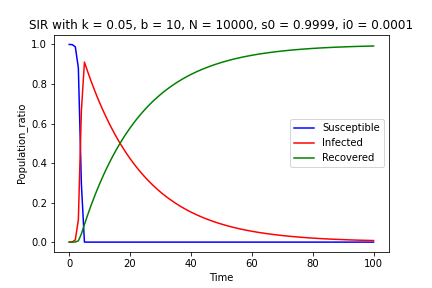
\includegraphics[scale=0.8]{sir_discrete_simulation0.png}
    %     \caption{A simulation of discrete SIR model.}
    %     \label{fig:discrete_simulation0}
    % \end{figure}
    
    Next, we investigate whether the discrete model agrees or disagrees with the continuous model on reproducing the efficacy of social distancing on slowing down the spread of infectious disease. Running the same simulation with the parameter b now set to 1 instead of 10, as in ODE social distancing simulation, we obtain Figure \ref{fig:discrete_simulation1}, which is qualitatively very similar to Figure \ref{fig:discrete_simulation1}. This tells us that social distancing is an effective measure in fighting the infectious disease by 'flattening the curve'.

    % \begin{figure}[h]
    %     \centering
    %     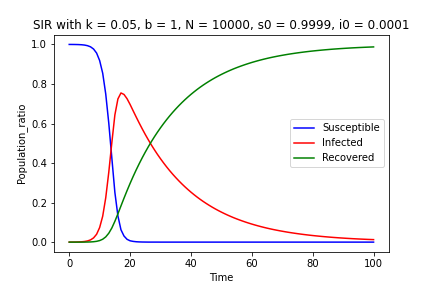
\includegraphics[scale=0.8]{sir_discrete_simulation1.png}
    %     \caption{A simulation of discrete SIR model in a ``socially distanced'' society.}
    %     \label{fig:discrete_simulation1}
    % \end{figure}
    
    We can also use discrete model to investigate how \(b\) and \(k\) can affect the dynamics of the system. First, we look at the time for all people being infected ($s(t) = 0$). From the phase diagram in Figure \ref{fig:phase_transition_full_infection_discrete}, we can draw the similar conclusion as the ODE version that large \(b\) and small \(k\) lead to the decrease of time for full infection. The major difference between discrete and ODE results is the phase boundary. For discrete model, the boundary is more step-like and have more sudden changes along \(b\) and \(k\) axis. This is again due to the discrete change of data in discrete model. 
    
    % \begin{figure}[h!]
    %     \centering
    %     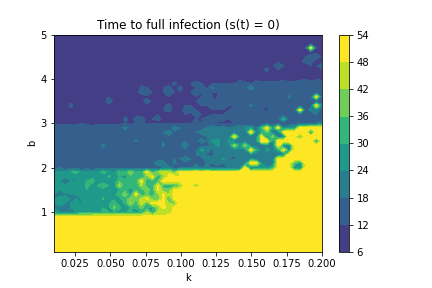
\includegraphics[scale=0.8]{phase_transition_full_infection_discrete.png}
    %     \caption{Phase diagram relating parameters and time to full infection for discrete model.}
    %     \label{fig:phase_transition_full_infection_discrete}
    % \end{figure}
    
   Finally, we can take a further look at the scenario where the infected people prevail in number($i(t) > 0.5$). Similar to Figure \ref{fig:phase_transition_outnumber}, we can see that the phase boundary for discrete model, as shown in Figure \ref{fig:phase_transition_outnumber_discrete}, shifts towards smaller \(b\) and larger \(k\) values, which again indicates that there are some instances where $i(t) > 0.5$ is fulfilled while $s(t) > 0$.
    
    % \begin{figure}[h!]
    %     \centering
    %     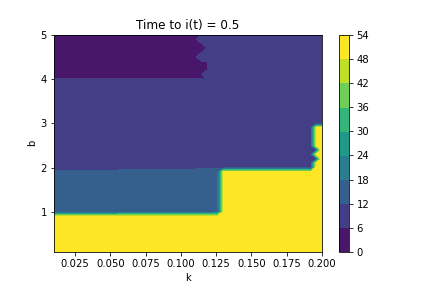
\includegraphics[scale=0.8]{phase_outnumber_discrete.png}
    %     \caption{Phase diagram relating parameters and time to \(i(t) > 0.5\) for discrete model.}
    %     \label{fig:phase_transition_outnumber_discrete}
    % \end{figure}

    \section{Spatial SIR model} \label{section:spatial_SIR}

    \subsection{PDE model} \label{section:spatial_SIR_pde}

    As discussed in Section \ref{section:intro}, the basic SIR model posits that any individual can interact with any other individual in the population. This is not a realistic assumption since we know that individuals generally only interact with people who are spatially nearby. We implement the PDE model to investigate how the diffusion weight \(p\) and the initial conditions qualitatively affect the infection dynamics. In order to get interesting dynamics, we fix the ``communicability" parameter \(b = 1\) and the ``recovery" parameter \(k = 0.075\) using our results from the ODE model in Section \ref{section:SIR_model}. We make this choice of parameters as it is close to the phase transition boundary in Figure \ref{fig:phase_transition_full_infection}. We also take \(M = 200\), and so our population lives in a \(200 \times 200\) two-dimensional grid.

    We first investigate how the infection dynamics change with the diffusion weight \(p\). We consider the initial condition in which only the center point of the grid is fully infected and all other points are fully susceptible. The PDE is simulated from this initial condition for \(0 \leq t \leq 500\). At \(t = 500\), we calculate the fraction of the population that had been infected at some time point, which is easily computed by \(1 - \frac{1}{M^2} \sum_{x} s(x, 500)\). Note that \(s(x,t)\) roughly denotes the fraction of the population at point \(x\) that is susceptible at time \(t\). By varying the diffusion weight \(p\) and examining the above measure, we get a sense for how the diffusion weight affects how fast the infection spreads through the grid. Our results are shown in Figure \ref{fig:infection_vs_p}.
    
    \begin{figure}[h!]
        \centering
        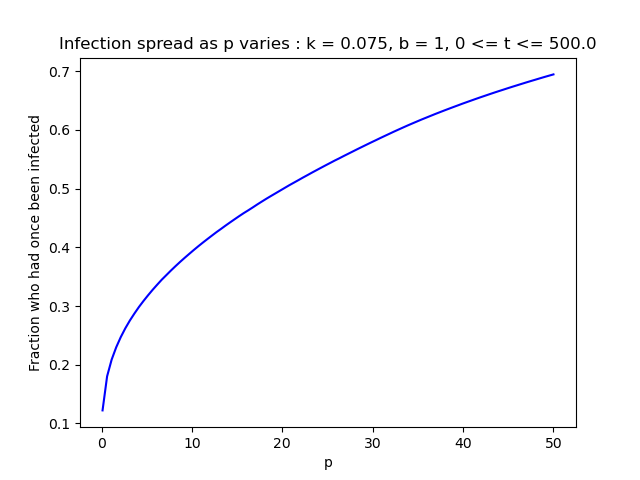
\includegraphics[scale=0.45]{infection_vs_p.png}
        \caption{Infection dynamics across the grid as diffusion weight \(p\) varies.}
        \label{fig:infection_vs_p}
    \end{figure}

    Examining Figure \ref{fig:infection_vs_p}, we see that the fraction of the population who had once been infected increases as \(p\) increases, agreeing with our intuition that the infection spreads faster with larger diffusion weight. However, strikingly the second derivative of the curve is negative. This result can be interpreted to have policy implications. For example, if a law is passed that only shuts down a few institutions during a pandemic (e.g. only gyms and sports centers) while all other institutions are free to operate (i.e. \(p\) is large), then we shouldn't expect the infected fraction to drop by much. So the marginal gain of closing just a few institutions is perhaps not worth the economic cost. However, if a law was passed to close down most institutions (i.e. when \(p\) is small), then further more stringent laws will have a greater affect on the infected fraction.
    
    We now investigate how the initial conditions qualitatively affect the infection dynamics. In particular, we compare the scenarios in which only the center point is fully infected and when only the upper left corner is fully infected. Again, we run the simulation using \(k = 0.075, b = 1, M = 200\). Using our result from Figure \ref{fig:infection_vs_p}, we used \( p = 25\) in order for the infection to spread fast enough so that there are qualitative differences in the dynamics. A snapshot of the dynamics is presented in Figures \ref{fig:pde_center} and \ref{fig:pde_corner} (found in Appendix \ref{appendix:sir_pde}). The plots clearly show different susceptibility across the population based on initial condition. When the initial infection is in the corner, there are fewer directions the infection can spread (some directions are blocked by the boundaries of the grid). In contrast, the infection beginning at the center of the grid can spread in all directions due to diffusion behavior. 
    
    \subsection{Agent-based model}
    We now turn to the agent-based model and ask similar questions as above. In this model, each agent is assigned with a random real-valued coordinates \( (x_{i},y_{i}) \in [0,1]\times[0,1]\) representing their initial position. In each time step, they move by length p in a random direction and interact with agents within radius \(q\). Based on the phase diagrams from the agent-based model in Appendix \ref{appendix:sir_discrete_figs}, we picked \(b=1\) (from which we compute \(q = \sqrt{b/(N\pi)}\)) and \(k=0.075\) and ran simulations with different \(p's\) ranging from 0 to 0.02, but holding other variables constant (population \(N = 10,000\) and initial infection rate \(i_{0}=0.0001\)). 
    \begin{figure}[h]
        \centering
        \begin{minipage}[b]{0.4 \textwidth}
            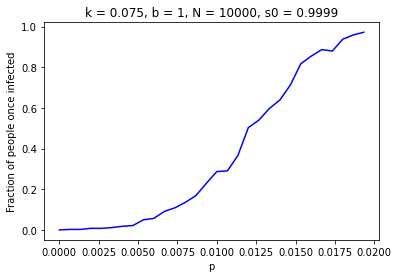
\includegraphics[width=\textwidth]{./spatial_model/infected_p.png}
            \caption{}
            \label{fig:agent_p}
        \end{minipage}
        \hfill
        \begin{minipage}[b]{0.45 \textwidth}
            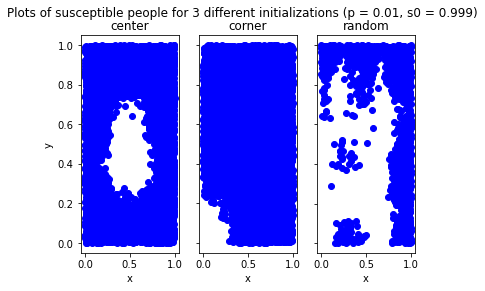
\includegraphics[width=\textwidth]{spatial_model/effects_initialization.png}
            \caption{}
            \label{fig:center_vs_corner}
        \end{minipage}
    \end{figure}
    
    As we can see from Figure \ref{fig:agent_p}, as infected agent travels a longer distance \(p\) for each time step, there are more agents who get infected throughout the simulation. This is consistent with our intuition that longer travel distances will result in contacting with larger number of yet-unaffected, susceptible agents, increasing the number of possible new infections.
    We next asked how the location of initial infection outbreak will influence how disease might spread. Figure \ref{fig:center_vs_corner} shows the results when three initially infected individuals were positioned around the center, at a corner or randomly distributed, respectively. The figure confirms our intuition that the larger the total area of possible contacts (in our example \(Area(\bigcup_{i=1}^{3} B_{q}(x_{i}, y_{i}))\): area of the union of three balls of radius q captured within the \([0,1]\times[0,1]\)) and the more towards the center initial outbreak occurs, the faster the disease will spread.   

    \section{Reinfection and spatial structure: a continuous SIRS model}\label{section:SIRS_model}

    \subsection{Steady state infection in the SIRS ODE model}
    Many diseases do not grant immunity to those who have recovered after being infected. Those who have been infected once by one strain can be infected again with another mutated strain. In principle, it's possible that the disease never dies out. One can then pose the qualitative question: What is the relationship between the steady state infection levels and the strain mutation rate and individual interaction frequency?
    
    To model reinfection, we can modify the SIR model to obtain the SIRS model in which recovered individuals can transition to the susceptible group. We introduce a new parameter \(m\) to denote the rate at which recovered individuals become susceptible \cite{brauerCompartmentalModelsEpidemiology2008}. (Here, \(m\) stands for mutation with the interpretation being that recovered individuals become susceptible as the pathogens mutate.) Modifying the SIR model, we obtain the following system of coupled differential equations 
    \begin{align*}
        s'(t) &= -b\cdot s(t) \cdot i(t) + m\cdot r(t) \\
        i'(t) &= b \cdot s(t) \cdot i(t) - k\cdot i(t) \\
        r'(t) &= k \cdot i(t) - m \cdot r(t).
    \end{align*}
    The parameters \(b\) and \(k\) retain their interpretation from the original SIR model presented in Section \ref{section:intro}. To cast our earlier questions in the context of this model, we can ask the following question. How do the parameters correspond to the long term steady state behavior of \(i(t)\)? 
    
    In order to simplify our investigation, we fix \(k = 1\) and investigate the long-term behavior of \(i(t)\) with respect to the pair \((b, m)\). Through some preliminary investigation, we decided to focus on the range \(2 \leq b \leq 10\) and \(0.001 \leq m \leq 7\) to illustrate interesting dynamical regimes. We discretize each interval into \(500\) grid points. Through the preliminary investigation, we found that with an initial condition of \(i(0) = 0.0001, s(0)=r(0)=0\), the simulated trajectories of \(s(t), i(t), r(t)\) generally reach their steady state by \(t = 50\), and so we take the steady state infection level to be given by \(i(50)\). Varying the parameters \((b, m) \in [2, 10] \times [0.001, 7]\) and simulating the SIRS ODE, we obtain the phase transition diagram for the steady state infection levels in Figure \ref{fig:sirs_ode_steady_state}. To give a richer picture of the dynamics, we present the phase diagram for the same parameter configurations of the peak infection levels in Figure \ref{fig:sirs_peak_infection}.

    \begin{figure}[h]
        \centering
        \begin{minipage}[b]{0.35 \textwidth}
            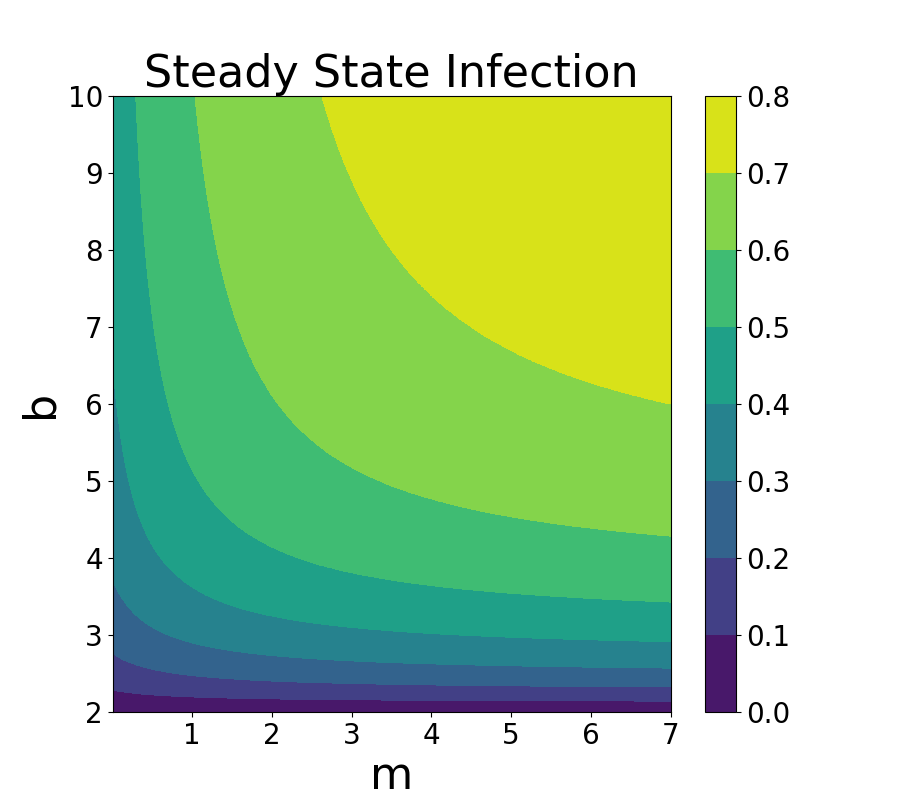
\includegraphics[width=\textwidth]{./sirs_variation/sirs_ode_infection_steadystate.png}
            \caption{}
            \label{fig:sirs_ode_steady_state}
        \end{minipage}
        \hfill
        \begin{minipage}[b]{0.35 \textwidth}
            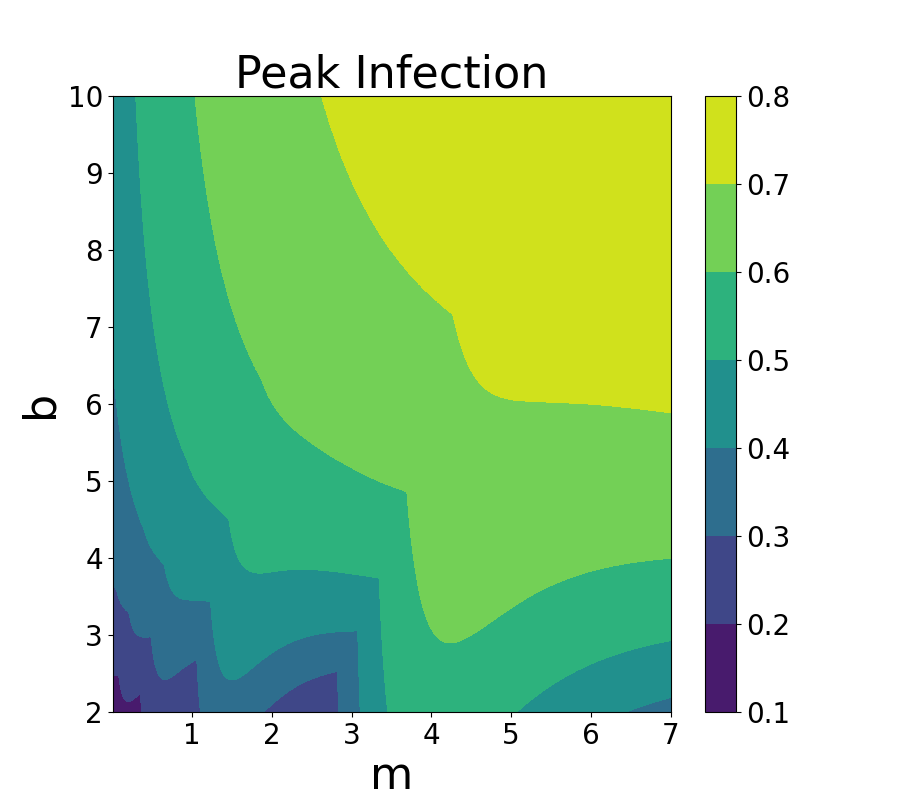
\includegraphics[width=\textwidth]{./sirs_variation/sirs_ode_peak_infection.png}
            \caption{}
            \label{fig:sirs_peak_infection}
        \end{minipage}
    \end{figure}

    Interestingly, Figure \ref{fig:sirs_ode_steady_state} indicates that all proportions are possible as steady state infection levels. It is very striking that the level sets of the steady state infection level form hyperbolas. Thus, for a fixed value of \(b=b^*\), there exists an interval \(J(b^*)\) such that the steady state infection rate is constant for all \(m \in J(b^*)\) (the reverse also holds). This result has policy implications when we interpret \(b\) as a measure of ``social distancing''. The phase diagram indicates that for a fixed mutation rate \(m\), reducing the steady state infection rate will require a \emph{large} decrease in \(b\), meaning that policies need to be severe; weak policies that reduce \(b\) by a tiny bit won't change the steady state infection level.

    Examining Figure \ref{fig:sirs_peak_infection} gives a richer picture of the disease dynamics. We see that for small values of \(m\) (i.e. \(m \leq 1\)), the peak infection level roughly matches the steady state infection level for any value of \(b\), indicating that infection level monotonically increases to its steady state level through the course of the simulation. However, once \(m\) starts to increase, there is a substantial change in the dynamics, especially for \(m \geq 4\). We see that the peak infection level is higher than the steady state infection level (especially so for small values of \(b\)). This result has policy implications. Severe restrictions aimed at reducing \(b\) should be continuously implemented even if the infection level seems to be rising at the current point in time; though the peak infection might be high for small values of \(b\), the steady state values are low. These policies shouldn't be abandoned just because there is a current spike in the infection level; the infection level will eventually settle to a lower level.

    A limitation of this model is that the rate at which individuals transition from the susceptible group to the infected group does not depend on the mutation rate \(m\). In reality, some mutuations give rise to more infectious or deadlier pathogens. In the context of our model, the parameters \(b\) and \(k\) should change when different strains of the pathogen arise. Future work should formulate a sensible model to capture this dependence and investigate the phase diagrams of steady state infection levels and peak infection levels. 

    \subsection{Travel restrictions versus social distancing in the spatial SIRS model}
    The continuous SIRS model stated above fails to account for the spatial structure in personal interactions discussed in Section \ref{section:intro}. We formulate a modification to the SIR PDE model and investigate the relative efficacy of travel restrictions versus social distancing in slowing down infection propagation speed. In the interest of brevity, these results and discussions can be found in Appendix \ref{appendix:sirs_pde}
    

    \section{The effects of `lock down' on disease spread: a discrete SIR model}\label{section:lock_down}
    
    \subsection{Spatial structure for discrete SIR model with 'lockdown' measure}
    In face of the outbreak of Covid-19, social distancing interventions or more strict 'lock down' measurements are introduced to slowdown the spread of the disease. To demonstrate the effects of 'lock down' on the dynamics of disease spread and shed light on the questions mentioned above, we propose to use a simple agent-based (discrete) SIR model to simulate the evolution of the disease.
    
    Due to the length limit, how the discrete model is improved to include spacial structure with 'lock down' measure and some results to characterize the model can be found in Appendix \ref{appendix:sirs_discrete}.
    
    To demonstrate the effects of 'lock down' measure, we change $T_0$ while keeping $D_0 = L/8$ and use $\lambda = 1$ as default value. Compare Figure \ref{fig:d=l/8} and \ref{fig:T0=2}, we can see when we introduce 'Lock down' at time 2 and people rapidly restricts their movement, the infection can be kept at a very low rate and majority of susceptible people can remain healthy. These results clearly show how an early and effective 'lock down' is able to help people fight the disease. However, when we look at the Figure \ref{fig:T0=2} and \ref{fig:T0=5}, we can see for a highly infectious disease (large $b$), even if we are just a few days later to take decisive measures, the spread of disease is very hard to control and much more people will be affected. Besides the timing for 'lock down', how strictly people will follow the 'lock down' can also affect its effectiveness. This can be demonstrated by Figure \ref{fig:T0=2 and lambda=2.5}. Here, $\lambda$ is the parameter that characterizes how fast the $D_0$ decreases. Compared with Figure \ref{fig:T0=2}, as $\lambda$ increases, the peak of infection rate increases and less people remain healthy. This shows even if people just do not follow the 'lock down' measure in time, namely, the restriction of movement does not happen as quickly as planned, the measure will become much less effective. 
    
    Another finding worth noting here is that instead of 'lock down', some other mild measures can be used together to slowdown the spread. For example, comparing Figure \ref{fig:b} and \ref{fig:d=l/8}, we can see if we can make population less mobile such as avoiding large gatherings (reduce $D_0$) while reducing the probability of transmission by wearing masks (decrease $b$), we can also effectively slowdown the spread of the disease.
    
    \begin{figure}[h]
        \centering
        \begin{minipage}[b]{0.35 \textwidth}
            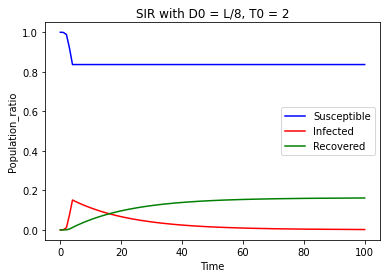
\includegraphics[width=\textwidth]{./discrete/sir_discrete_grid11.png}
            \caption{}
            \label{fig:T0=2}
        \end{minipage}
        \hfill
        \begin{minipage}[b]{0.4 \textwidth}
            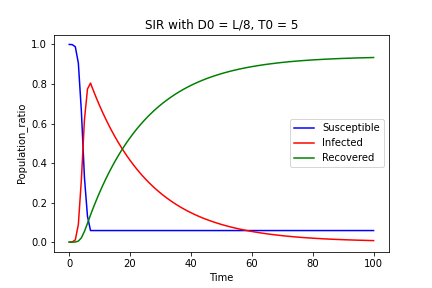
\includegraphics[width=\textwidth]{./discrete/sir_discrete_grid10.png}
            \caption{}
            \label{fig:T0=5}
        \end{minipage}
        \centering
        \begin{minipage}[b]{0.4 \textwidth}
            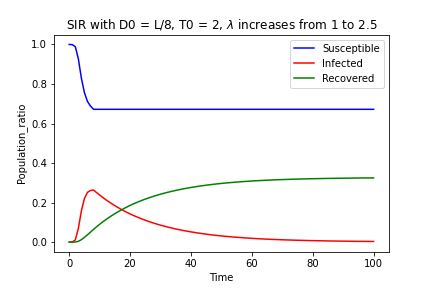
\includegraphics[width=\textwidth]{./discrete/sir_discrete_grid12.png}
            \caption{}
            \label{fig:T0=2 and lambda=2.5}
        \end{minipage}
        \hfill
        \begin{minipage}[b]{0.4 \textwidth}
            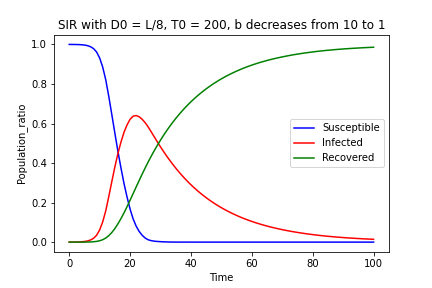
\includegraphics[width=\textwidth]{./discrete/sir_discrete_grid15.png}
            \caption{}
            \label{fig:b}
        \end{minipage}
    \end{figure}

    \subsection{Effects of lifting the 'lock down' measure too early}
    Furthermore, we can set a time $T_1$ when we release the 'lock down' measure and $D_0(T_1) = D_0$ to see how the pandemic will evolve if we end 'lock down' too early. From the Figure \ref{fig:T1}, we can find that if we lift the 'lock down' measure at $T_1 = 25$ (completely back to normal) when there are still enough infected people in the population, this highly infectious disease can still widespread and we can see a higher second peak occurs after $T_1$. This demonstrates that once a 'lock down' measure is in place, it is very important to decide when and how to lift this measure and make life become normal again.

        \begin{figure}[h]
        \centering
        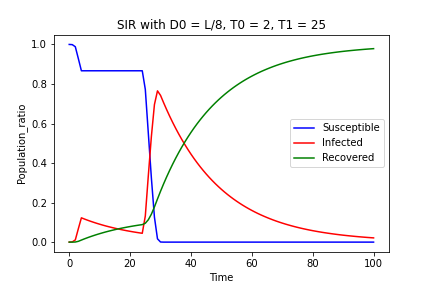
\includegraphics[scale=0.45]{./discrete/sir_discrete_grid14.png}
        \caption{Lifting 'lock down' measure too early may lead to second wave.}
        \label{fig:T1}
    \end{figure}
    
    \section{SIRV discrete model: Evolution of infectious disease spread in 2D space with and without vaccines}\label{section:vaccine}
    
    In this discrete variation, we investigate how vaccines might suppress the spread of infectious disease. We first demonstrate that the introduction of vaccines flattens the infection curve as expected. Next we attempt to explain how this can be achieved by visualizing the snapshots of the "geography" of the disease taken at different times.    
    
    To achieve this in a more realistic scenario, a few changes were made from the original discrete SIR model. First, we introduce 2D n by n square dense grid where each cell represents an agent with disease state and activity level. The activity level, which replaces the parameter \(b\) from the original model, ranges from 0 to 8 indicating each agent's maximum number of contacts with its neighboring agents in each time step. It is randomly assigned and stays constant throughout the simulation. The order in which agents make contacts is randomly determined in each time step. When vaccines are included in a simulation, a given number of random agents with "S" or "R" receive vaccines in each time step. Agents with state "V" (for vaccinated) are assumed to be immune to infection. Agents are assumed to recover from infected state at rate \(k\) = 0.05 as before. However, in contrast to the original model infection chance upon contact is \(50\%\) and reinfection is possible (to more realistically reflect Covid-19). 
    
    \begin{figure}[h]
        \centering
        \begin{minipage}[b]{0.4 \textwidth}
            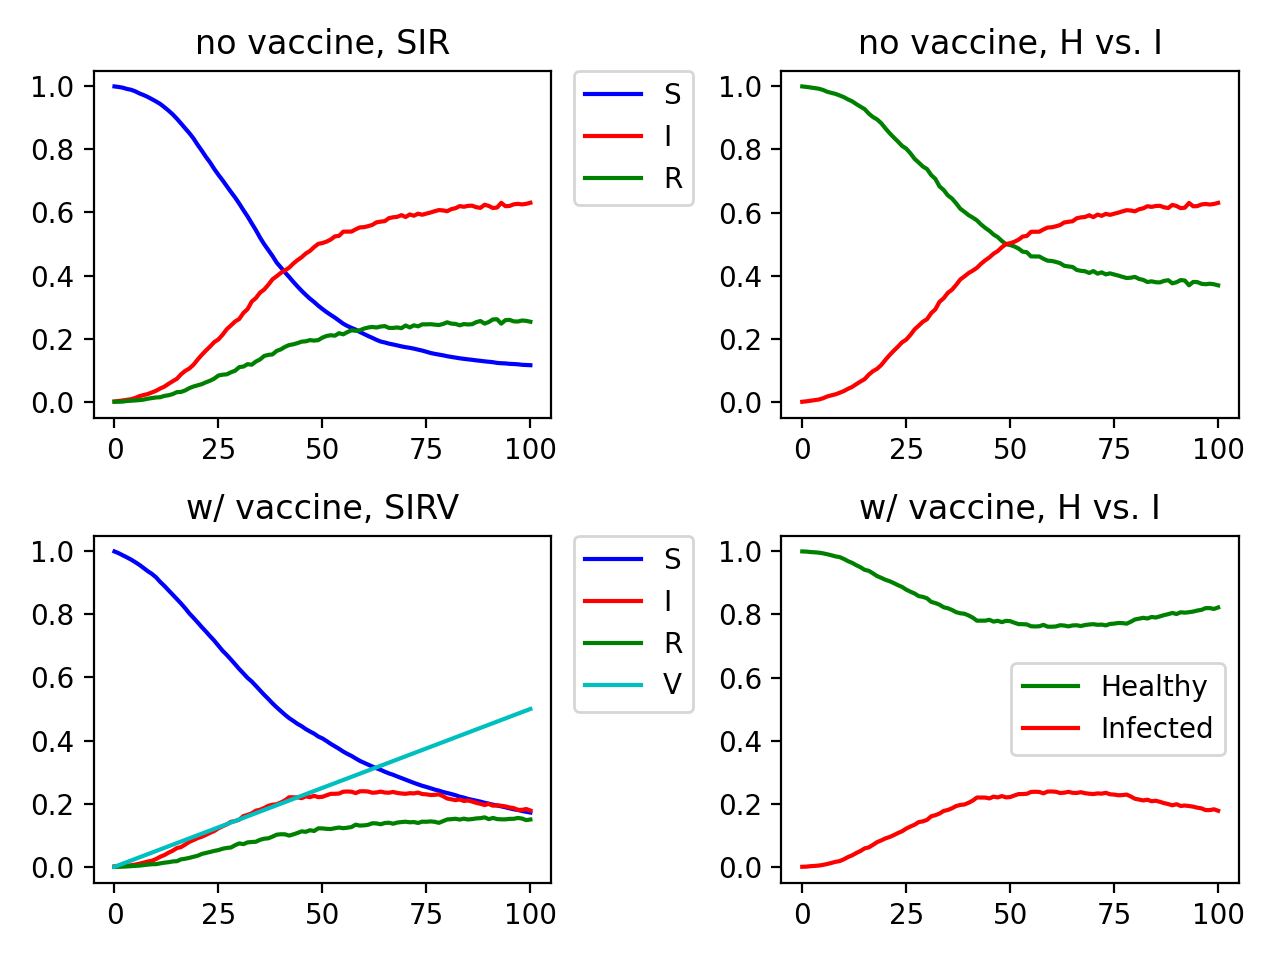
\includegraphics[width=\textwidth]{SIRV_1.png}
            \caption{}
            \label{fig:sirv1}
        \end{minipage}
        \hfill
        \begin{minipage}[b]{0.4 \textwidth}
            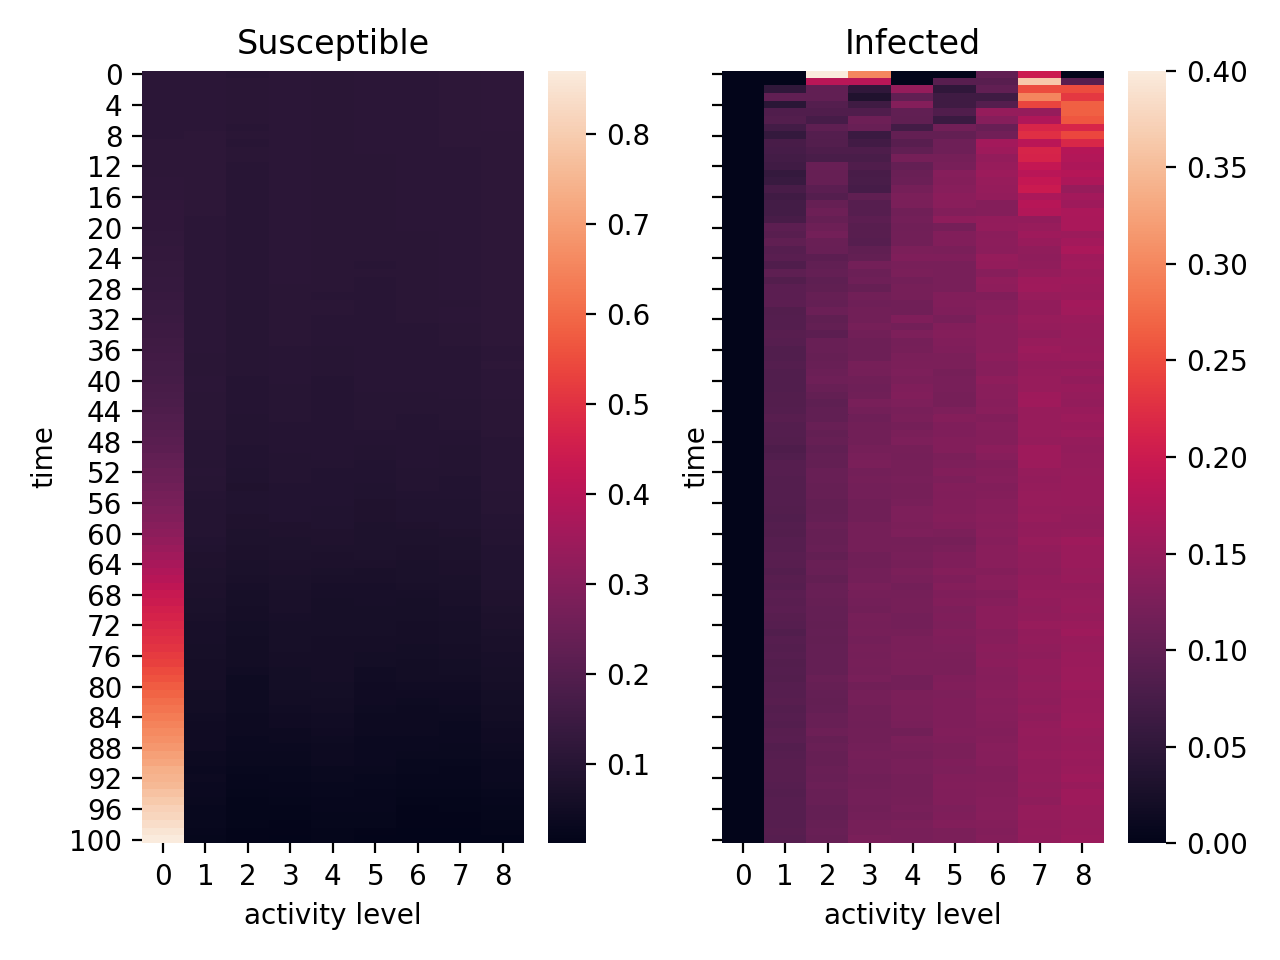
\includegraphics[width=\textwidth]{SIRV_2.png}
            \caption{}
            \label{fig:sirv2}
        \end{minipage}
        
    \end{figure}
    \noindent {\footnotesize
    \textbf{Figure \ref{fig:sirv1}} Evolution of SIR(V) states and Healthy vs Infected (Left/Right) under no-vaccine and with-vaccine conditions (Upper/Bottom) \textbf{Figure \ref{fig:sirv2}} Distribution of activity levels among the susceptible (left) and infected agents (right) under no-vaccine condition\par}
    \vspace{5mm}
    From Figure \ref{fig:sirv1}, we see that distributing vaccines even at the seemingly slow rate of 0.005 (\(0.5\%\) of the population receive vaccines in each time step) is very effective in flattening the infection curve early on, and large majority of the population remains unaffected ('Healthy' on the right panels indicating the fraction of agents with SRV states combined) by the disease, making a striking contrast with the no-vaccine condition. Figure \ref{fig:sirv2} confirms our intuition that infections are confined to relatively more active agents, explaining why infection curves on the upper panels starts plateauing at around 0.6.  
    
    To gain further insight into how vaccines might help retard the spread of infectious disease, we visualize how "geography of infection" in the 2D grid changes over time. To achieve this, state of individual agents was tracked throughout the simulations and averaged over every 10 time steps. Each agent is either healthy (0) or infected (1) in each time step and averaging this score over 10 time steps produces numbers between 0 and 1. The resulting average scores is plotted as heatmaps as shown in Figure \ref{fig:sirv3} and Figure \ref{fig:sirv4}.
    
    A close examination of these two figures reveals that the vaccinated agents act as seeds that help form small local patches of healthy individuals that progressively grow in size. Interestingly, in the latter half of the simulation we observe that vaccines also help prevent the disease from expanding its territory at a more global scale (compare bottom panels of Figure \ref{fig:sirv3} and Figure \ref{fig:sirv4}). This may allow large regions of unaffected agents to remain unaffected, a possible explanation for how even a slow distribution of vaccines can be very effective in flattening the curve.      
    
     \begin{figure}[h]
        \centering
        \begin{minipage}[b]{0.4 \textwidth}
            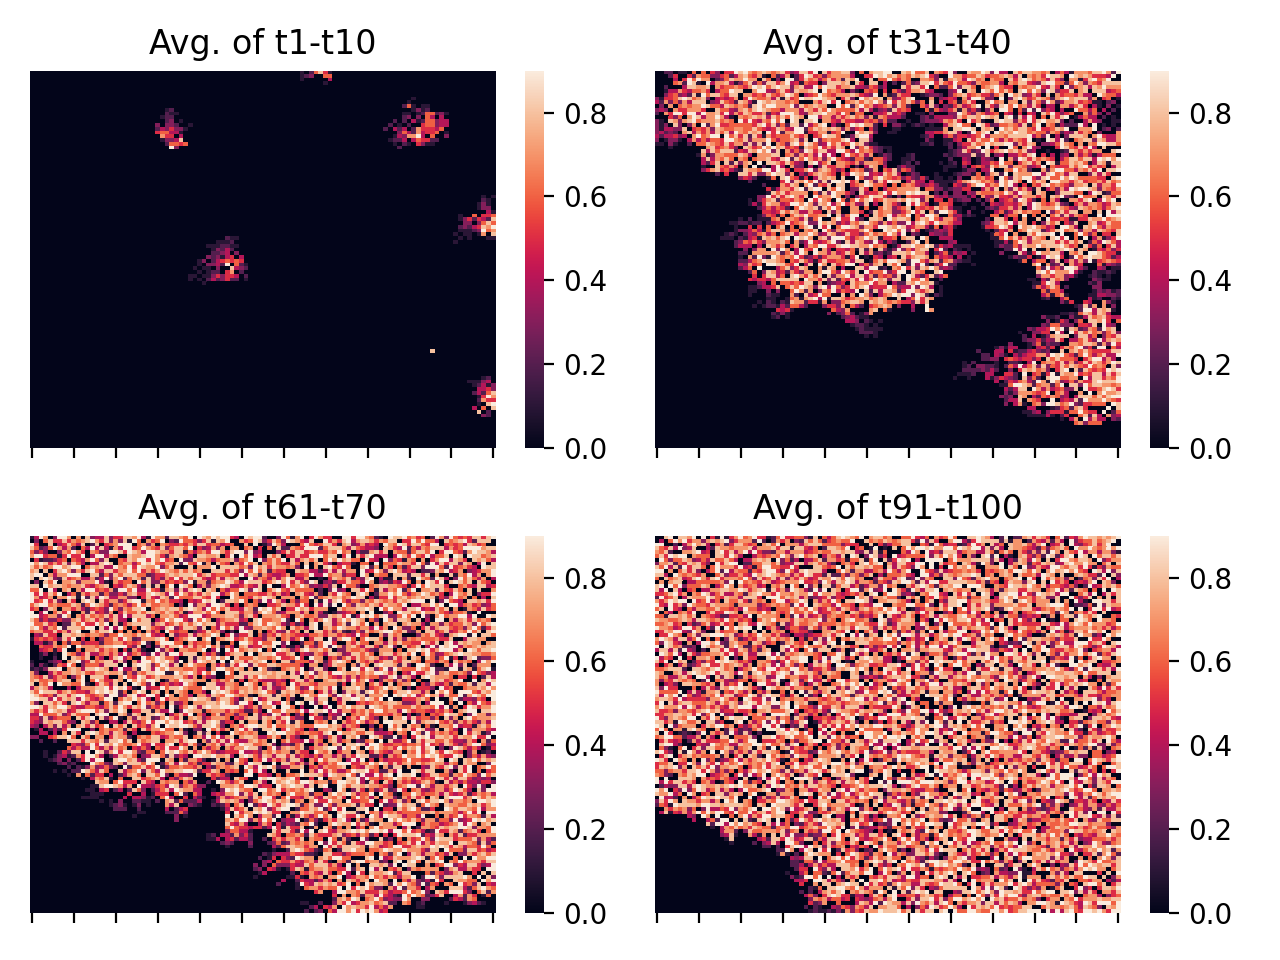
\includegraphics[width=\textwidth]{SIRV_3.png}
            \caption{}
            \label{fig:sirv3}
        \end{minipage}
        \hfill
        \begin{minipage}[b]{0.4 \textwidth}
            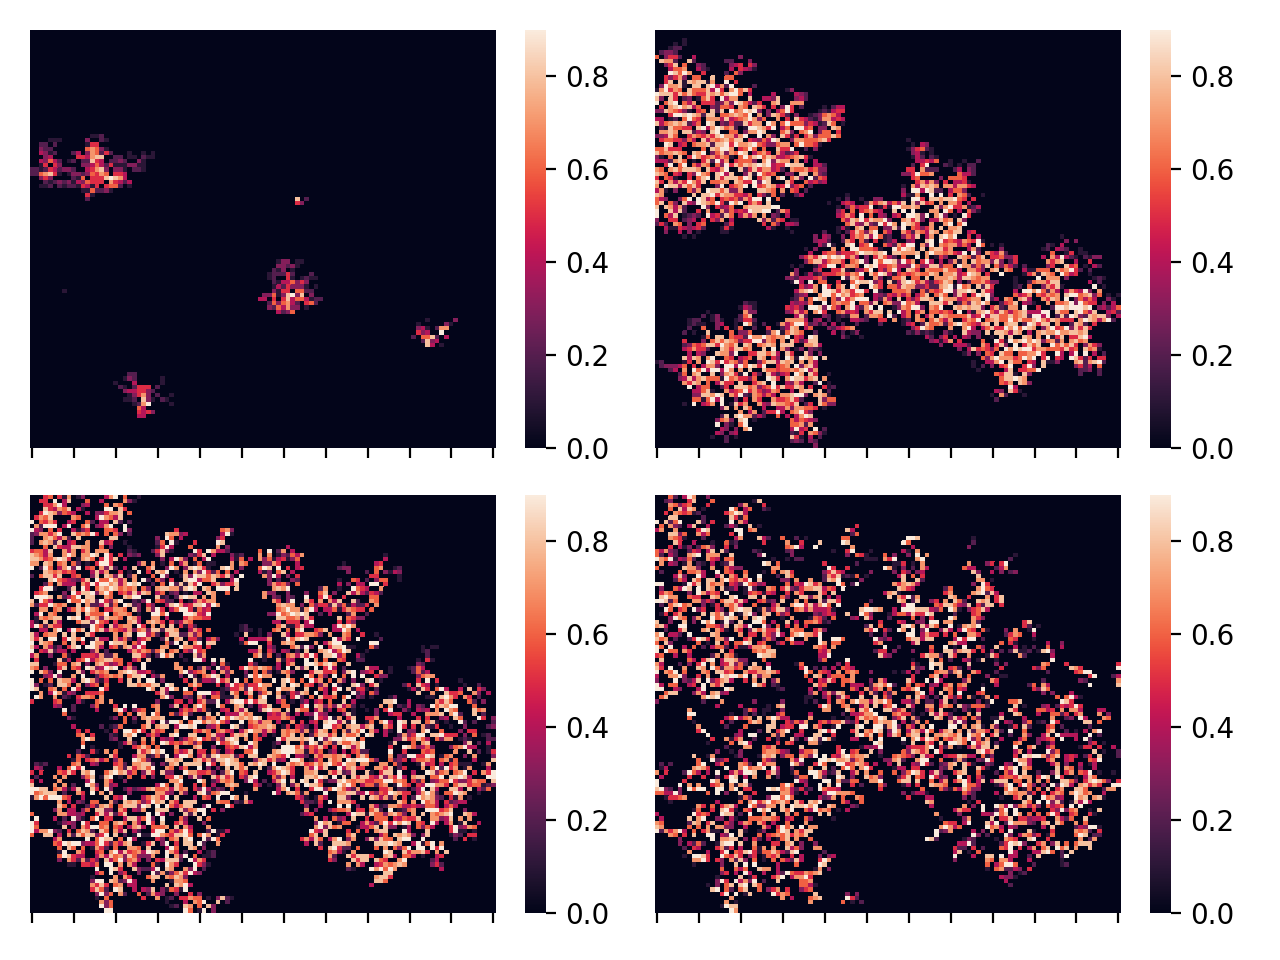
\includegraphics[width=\textwidth]{SIRV_4.png}
            \caption{}
            \label{fig:sirv4}
        \end{minipage}
        
    \end{figure}
    \noindent {\footnotesize
    \textbf{Figure \ref{fig:sirv3}} State grid averaged over 10 time steps under no vaccine (Upper: average over (\(t_{1}  t_{10}\)), (\(t_{31} ~ t_{40}\)), Bottom: average over (\(t_{61} ~ t_{70}\)), (\(t_{91} ~ t_{100}\)). 0 means an agent was healthy throughout 10 time steps whereas 1 means an agent remained infected throughout 10 time steps \textbf{Figure \ref{fig:sirv4}} Same as Figure \ref{fig:sirv3}, but with vaccine \par}
    \vspace{5mm}
    
    Thus, a possible future direction could be investigating a more concrete mechanism by which small patches of vaccinated agents might effectively suppress global spread of disease.

    \section{SIR model that depends on current state}\label{section:current_state}
    In reality, a single system of odinary differential equation might not accurately capture the patterns in changes of \(s(t)\), \(i(t)\) and \(r(t)\) throughout the process. For example, when a significant size of the population are infected, the government intervention and media exposure to the virus may potentially alter people's behavior. Moreover, after medical supplies are allocated and feasible treatment has been found, infected people may recover quicker. We can formulate such phenomena by introducing changes in values of parameters \(b\) and \(k\) to the systems of differential equations once \(i(t)\) or \(r(t)\) reaches a certain threshold. The system of equation now becomes
    \begin{align*}
        s'(t) &= -b'\cdot s(t) \cdot i(t) \\
        i'(t) &= b'\cdot s(t) \cdot i(t) - k'\cdot i(t) \\
        r'(t) &= k'\cdot i(t)
    \end{align*}
where $b' < b$ and $k' > k$ in the discussion above. In practice, we can set an event, such as  \(i(t) = 0.3\), that terminates the ode simulation, Then, we run a new simulation with the altered parameters for the remaining time interval starting at the state that is left off by the previous simulation. Further analysis would be based on the concatenated solution of the systems. Note that the following discussion of models in this section all take $k = 0.05$, $b = 0.8$ and $i=10^{-6}$ as initial condition. Figure \ref{fig:Sharp} in Appendix \ref{appendix:sir_continous} helps to illustrate how the simulation behaves when we introduce such abrupt change in parameters along the way. The sharp turn on the left correponds to the first event at time $t$ when \(i(t) = 0.3\), which is set to alarm the public when there is large number of population infected. After reaching this state, the $b'=0.1$ will be active for the rest of the simulation. Similarly, another event is set when \(r(t) = 0.4\), in which the $k'$ that will be effective for the rest of the simulation is doubled. We now focus on the event that will alter the values of b. We may want to know, given a fixed initial condition, the relationship between the time such event takes place and the peak of infected population throughout the simulation. The result may be informative to policy makers as the maximum infected rate should not exceeds the capcity of the medical system. In this case, we consider a variety of events that have distinct values of $b2$ for the second stage of simulation. Note that smaller $b2$ value would intuitively means stricter policies or more active response to the event, and it is not surprising that smaller $b2$ values would lead to lower maximum infected population size. 
\begin{figure}[h]
        \centering
        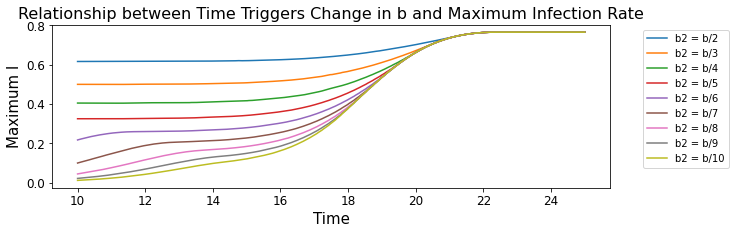
\includegraphics[scale=0.4]{./b_and_max_i.png}
        \caption{Relationship between Time of Event and Max Infection Rate}
        \label{fig:T3}
\end{figure}
From Figure \ref{fig:T3}, it is clear that after the 20th day since the outbreak, these events would have little impact on the peak of infected population size. Intuitively, if emergency responses towards the disease take place too late, then the infected population would reach its maximum size naturally. The left part of the plot shows that if such event takes place early, then the maximum infected rate through out the process would be kept relatively low, and mainly determined by the value of $b'$ . The intuition is that $b'$ is much smaller than $b$, and it is active in the simulation soon after the outbreak when the infected poopulation is relatively small. Another take away is that, even though stricter policies would typically have better outcome over keeping the maximum infected population size lower, its advantage would be less effective when the infected population starts to blow up in time. In this plot, between the time interval of $[16, 20]$ the curves start to converge and the difference between their ability to cap maximum infected population size down soon vanishes. For all events that have power to cap the maximum infected population under half of the total population size in this plot, the last day to activate changes in $b$ is approximately day 19, in which case there are no significant comparative advantage in having better policies. Hence, when the infected population starts to blow up, acting promptly is more important than spending time coming up with better responses. 


    \section{Conclusion}
    The original SIR and spatial SIR models are simple, interpretable models for disease spread. While they don't account for a lot of nuance in real world infection dynamics, one can easily get a rough picture of how disease will spread in different settings. In Section \ref{section:SIR_model}, we obtained phase diagrams for the SIR model that indeed showed that strict social distancing measures (small values of \(b\)) can result in disease dynamics in which some individuals are never infected even when recovery rates are small (i.e. small \(k\)). In Section \ref{section:spatial_SIR}, we showed that the total infection level seems to grow logarithmically in the diffusion weight; the main policy conclusion is ``all or nothing'', meaning that policy must be strict in order to have a strong effect (see Section \ref{section:spatial_SIR}).

    We extended these simple models to investigate nuances in disease dynamics under more complicated settings. In Section \ref{section:SIRS_model}, we investigated reinfection due to mutations of the pathogen. We showed that there are parameter configurations of the mutation rate \(m\) and interaction rate \(b\) in which the disease remains endemic and that the level sets form hyperbolas; the policy implications are outlined in Section \ref{section:SIRS_model}. We also investigated the relative efficacy of travel restrictions versus social distancing in reducing the infection propagation speed in a spatial model of reinfection (Appendix \ref{appendix:sirs_pde}). We concluded that travel restrictions are much more effective.
    
    In Section \ref{section:lock_down}, we studied how the 'lock down' measure could change the dynamics of disease spread via discrete SIR model. We demonstrated that the larger the area a person could access, the faster the disease could transmit. Thus, with an effective 'lock down', namely, confine people in a smaller space, the infection rate can be slowed down and more people can remain healthy. However, we also found an early lifting of 'lick down' could lead to a second wave and how strictly people followed the measure strongly affected its effectiveness.

    In Section \ref{section:vaccine}, we evaluated the impact of vaccines throughout the simulation. From the comparison between simulations with and without vaccines distribution, we found that even at a low rate of vaccine distribution, the presence of vaccine still contributes to the flattening of infection curve in a great deal. Taking into account of the spatial components, our visualization showed that vaccines not only helps to build local pathes of healthy individuals, but it also keep disease from spreading gloabally later in the simulation. Future studies might focus on investigating the mechanism behind how small patches of vaccinated agents effectively suppress global spread of disease.

    In Section \ref{section:current_state}, we looked into how events altering the values of parameters that take place in the middle of continuous simulation impact the maximum infected population size. We found that the difference in the ability of capping down the maximum infected population size would quickly vanish as the infected population start to blow up. This emphasizes the importance of acting promptly in terms of capping down the maximum infected population under the capacity of medcal system. A model with much more freedom of adjusting parameters throughout the simulation is discussed in Appendix \ref{appendix:sir_continous}. Further investigation may incorporate data in the real world and analyze the continuous changes in $b$ deeper.

    \newpage

    \appendix 
    \section{SIR ODE Model}\label{appendix:sir_ode_figs}
    The SIR ODE model is formulated with the following differential equations,
    \begin{align*}
        s'(t) &= -b\cdot s(t) \cdot i(t) \\
        i'(t) &= b \cdot s(t) \cdot i(t) - k\cdot i(t) \\
        r'(t) &= k \cdot i(t).
    \end{align*}
    Here \(s(t)\), \(i(t)\) and \(r(t)\) denote the fraction of the population residing in each corresponding category at time \(t\). The first equation indicates that the number of infections (transitions from the \(S\) category to the \(I\) category) positively related with \(s(t)\), \(i(t)\) and the parameter \(b\). Intuitively, more people are infected each day when there are more susceptible, infected, or more interactions. The third equation shows that the number of recoveries (transitions from the \(I\) category to the \(R\) category) is positively related with \(i(t)\) and the parameter \(k\). Intuitively, there are more recoveries when there are more infected or when the recovery rate is higher. The second equation can be seen as a result of the first and the third equation, as the sum of population of categories must be equal to the total population \(N\) at any given time. Figures \ref{fig:simulation0} and \ref{fig:simulation1} are the figures referred to in the discussion of the SIR ODE model. The phase diagrams presented in Figures \ref{fig:phase_transition_full_infection} and \ref{fig:phase_transition_outnumber} are also referred to in the discussion of the SIR ODE model. 
    
    \begin{figure}[h]
        \centering
        \begin{minipage}[b]{0.4 \textwidth}
            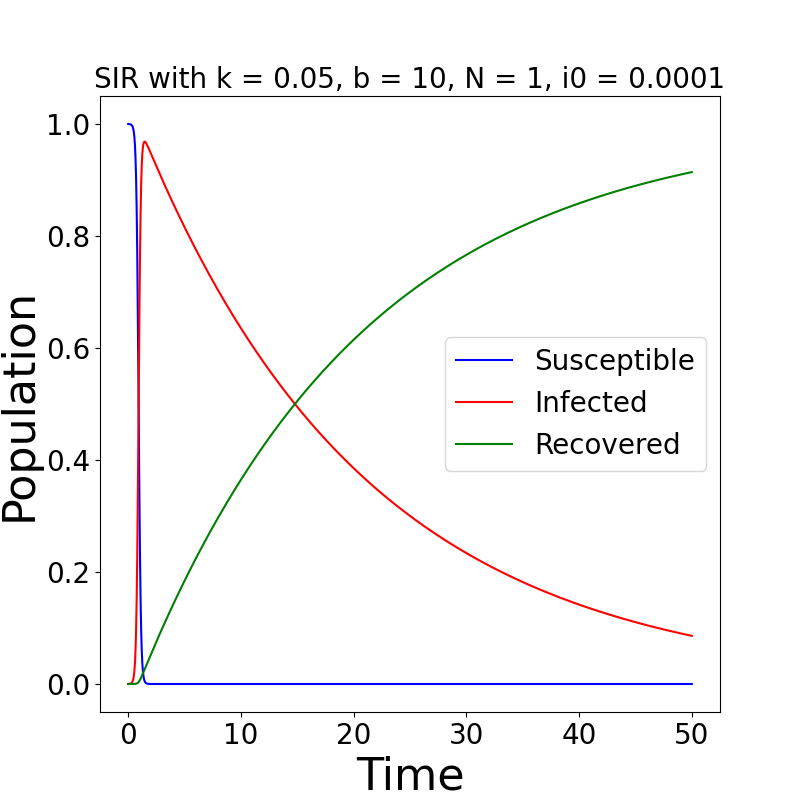
\includegraphics[width=\textwidth]{sir_ode_simulation0.png}
            \caption{}
            \label{fig:simulation0}
        \end{minipage}
        \hfill
        \begin{minipage}[b]{0.4 \textwidth}
            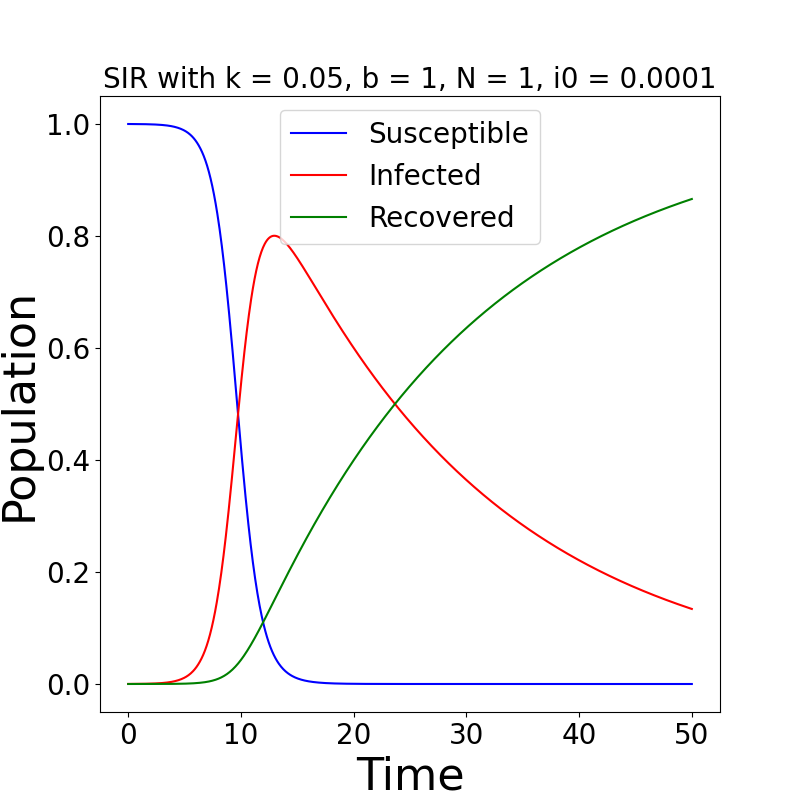
\includegraphics[width=\textwidth]{sir_ode_simulation1.png}
            \caption{}
            \label{fig:simulation1}
        \end{minipage}
        
    \end{figure}

    \begin{figure}[h]
        \centering
        \begin{minipage}[b]{0.4 \textwidth}
            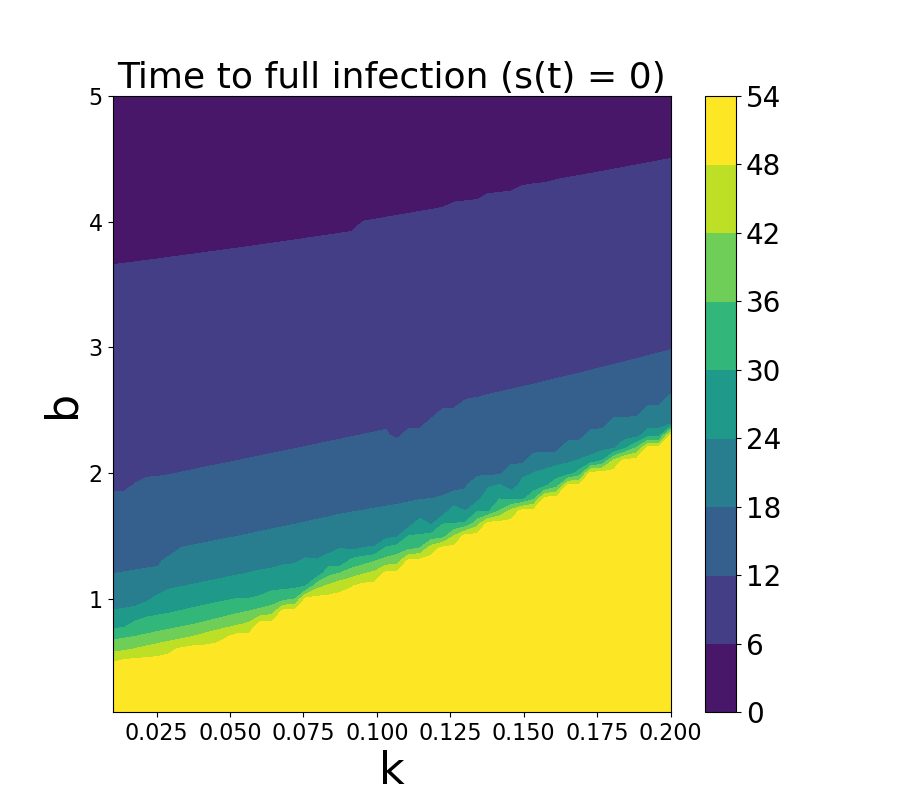
\includegraphics[width=\textwidth]{phase_transition_full_infection.png}
            \caption{}
            \label{fig:phase_transition_full_infection}
        \end{minipage}
        \hfill
        \begin{minipage}[b]{0.4 \textwidth}
            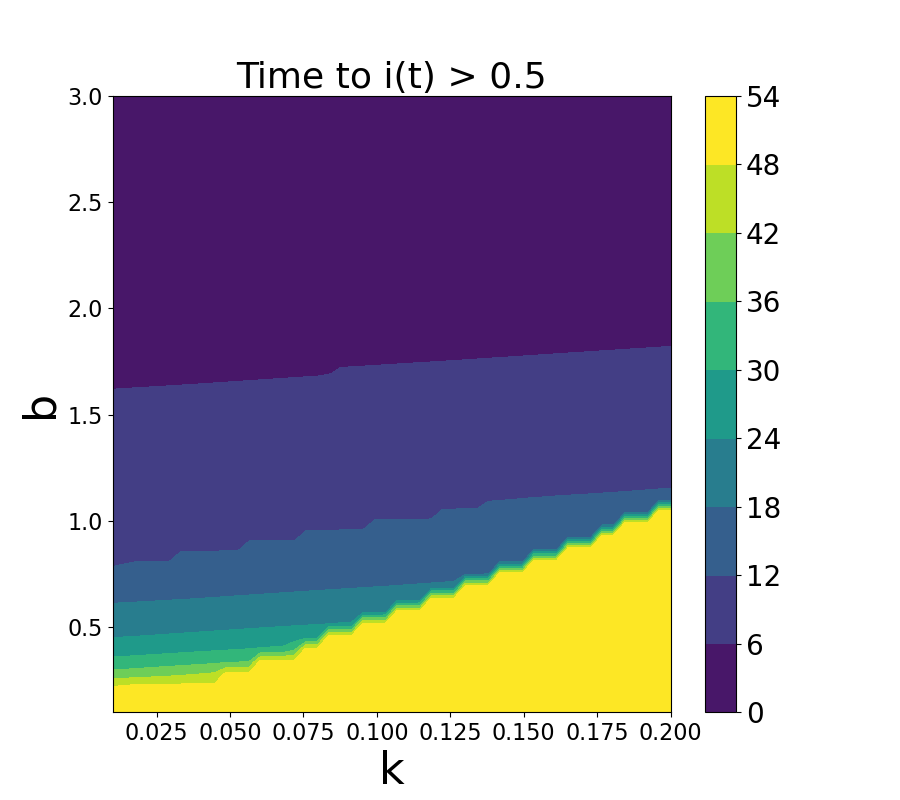
\includegraphics[width=\textwidth]{phase_transition_outnumber.png}
            \caption{}
            \label{fig:phase_transition_outnumber}
        \end{minipage}
        
    \end{figure}

    \newpage
    
    \section{SIR Discrete Model - Figures}\label{appendix:sir_discrete_figs}
    Figures \ref{fig:discrete_simulation0} and \ref{fig:discrete_simulation1} are the figures referred to in the discussion of the SIR ODE model. The phase diagrams presented in Figures \ref{fig:phase_transition_full_infection_discrete} and \ref{fig:phase_transition_outnumber_discrete} are also referred to in the discussion of the SIR ODE model.
    \begin{figure}[h]
        \centering
        \begin{minipage}[b]{0.4 \textwidth}
            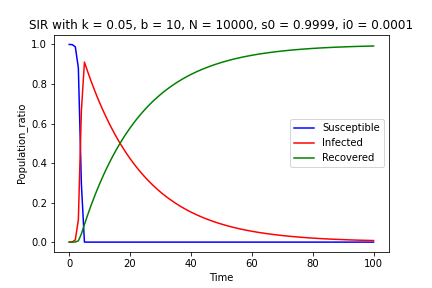
\includegraphics[width=\textwidth]{sir_discrete_simulation0.png}
            \caption{}
            \label{fig:discrete_simulation0}
        \end{minipage}
        \hfill
        \begin{minipage}[b]{0.4 \textwidth}
            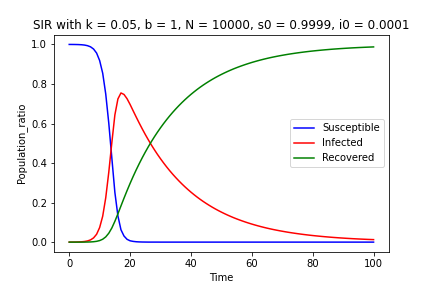
\includegraphics[width=\textwidth]{sir_discrete_simulation1.png}
            \caption{}
            \label{fig:discrete_simulation1}
        \end{minipage}
        
    \end{figure}

    \begin{figure}[h]
        \centering
        \begin{minipage}[b]{0.4 \textwidth}
            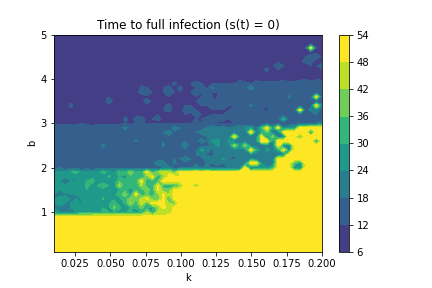
\includegraphics[width=\textwidth]{phase_transition_full_infection_discrete.png}
            \caption{}
            \label{fig:phase_transition_full_infection_discrete}
        \end{minipage}
        \hfill
        \begin{minipage}[b]{0.4 \textwidth}
            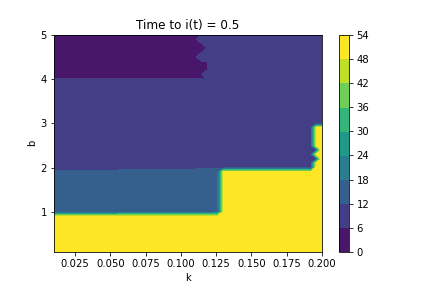
\includegraphics[width=\textwidth]{phase_outnumber_discrete.png}
            \caption{}
            \label{fig:phase_transition_outnumber_discrete}
        \end{minipage}
    \end{figure}

    \newpage 

    \section{Spatial SIR PDE Model}\label{appendix:sir_pde}
    The spatial SIR PDE model is formulated as follows. For time \(t\) and \(x \in [0, M] \times [0, M]\), we have
    \begin{align*}
        \frac{\partial s(x,t)}{\partial t} &= -b \cdot s(x, t) \cdot i(x, t) + p \cdot \Delta s(x, t) \\
        \frac{\partial i(x, t)}{\partial t} &= b \cdot s(x, t) \cdot i(x, t) - k \cdot i(x, t) + p \cdot \Delta i(x, t) \\
        \frac{\partial r(x, t)}{\partial t} &= k \cdot i(x, t) + p \cdot \Delta r(x, t)
    \end{align*}
    where \(\Delta\) denotes the Laplacian. The quantities \(s(x, t), i(x, t)\) and \(r(x, t)\) can be roughly thought of as ``densities'' of susceptible, infected, and recovered individuals at position \(x\) and time \(t\). 

    Figures \ref{fig:pde_center} and \ref{fig:pde_corner} are presented below. These figures were referenced in the discussion of Section \ref{section:spatial_SIR_pde}
    \begin{figure}[h]
        \centering
        \begin{minipage}[b]{0.45 \textwidth}
            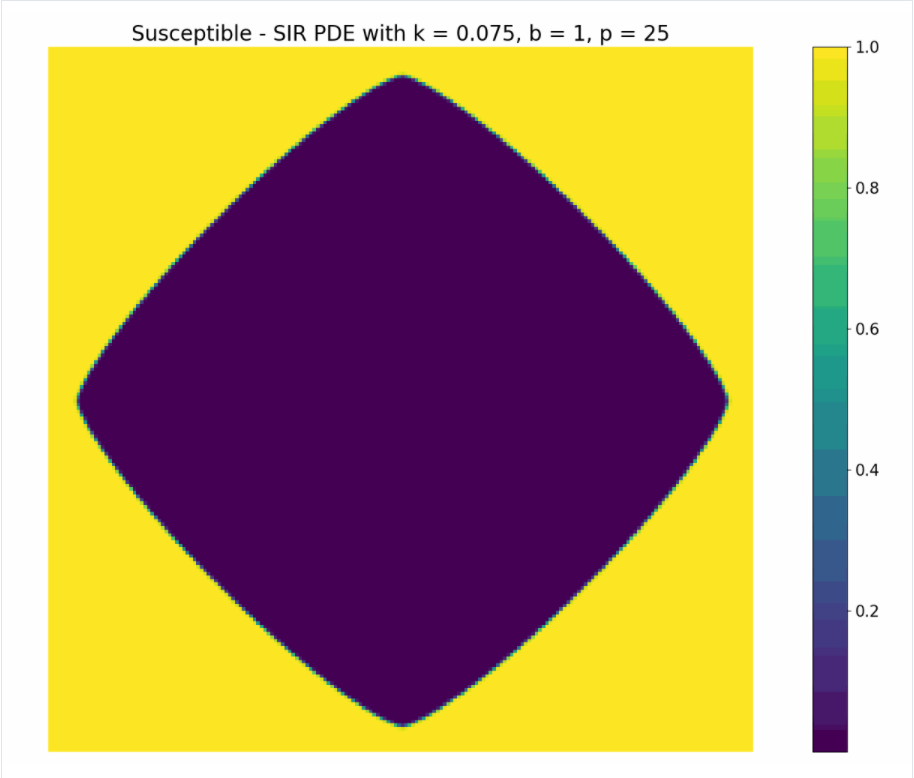
\includegraphics[width=\textwidth]{pde_center_susceptible_snapshot.png}
            \caption{}
            \label{fig:pde_center}
        \end{minipage}
        \hfill
        \begin{minipage}[b]{0.45 \textwidth}
            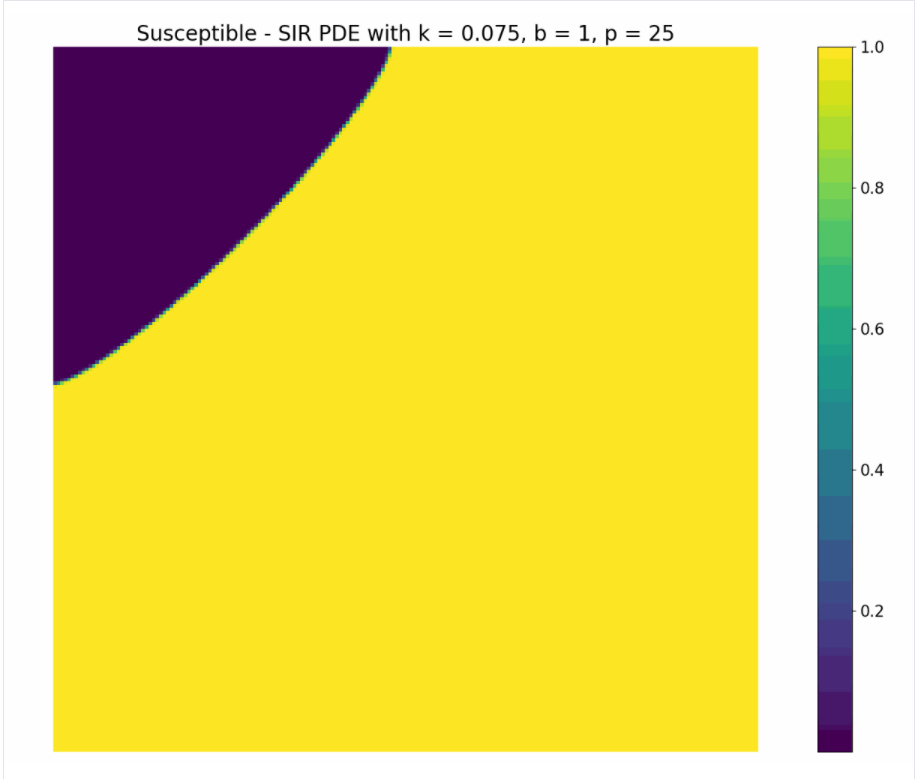
\includegraphics[width=\textwidth]{pde_corner_susceptible_snapshot.png}
            \caption{}
            \label{fig:pde_corner}
        \end{minipage}
    \end{figure}

    \newpage

    \section{Travel restrictions versus social distancing in the spatial SIRS model} \label{appendix:sirs_pde}
    As stated, the SIRS model fails to account for the spatial structure in personal interactions discussed in Section \ref{section:intro}. To account for this, we modify the the PDE model defined in Section \ref{section:intro} to obtain a spatial SIRS model. In the midterm proposal, we had proposed to study the spatial model defined in \cite{baileySimulationStochasticEpidemics1967}, which did not have a diffusion term but instead simply replaced \(i(x, t)\) with a kernel-average \(\int K(||y-x||) \, i(y, t) \, dy\). This simpler model is not as principled as the PDE model, which is the continuous limit after positing random walk movement. In contrast, the other model has no real mechanism for how the infection in nearby points affects the current point; taking a kernel-average results in a totally phenomenological model. Hence, we use the PDE model and modify it to obtain a spatial SIRS model. In particular, we obtain the following system of partial differential equations 
    \begin{align*}
        \frac{\partial s(x, t)}{\partial t} &= -b \cdot s(x, t) \cdot i(x,t) + m \cdot r(x, t) + p_s \cdot \Delta s(x, t)\\
        \frac{\partial i(x, t)}{\partial t} &= b \cdot s(x, t) \cdot i(x, t) - k \cdot i(x, t) + p_i \cdot \Delta i(x, t) \\
        \frac{\partial r(x, t)}{\partial t} &= k \cdot i(x, t) - m \cdot r(x, t) + p_r \cdot \Delta r(x, t)
    \end{align*}
    where \(p_s, p_i, p_r > 0\) are diffusion weights and the parameters \(b, k, m\) retain their interpretation for the SIRS ODE model. We intepret the parameter \(p_i\) to correspond to travel restrictions; light restrictions correspond to large values of \(p_i\) whereas severe restrictions correspond to small values of \(p_i\). We investigate the relative importance of social distancing vs travel restrictions in slowing down the spread of infection, i.e. what is the relationship between \((b, p_i)\) and the speed of propagation?
    
    To investigate these questions, we set \(k = 1\), \(p_s = p_r = 25 =: p\), and parametrize \(p_i = \gamma p\) for \(\gamma \in (0, 1)\). Informed by our results in Figures \ref{fig:sirs_ode_steady_state} and \ref{fig:sirs_peak_infection}, we fix \(m = 4\) to get illustrative dynamics. We then vary \(2 \leq b \leq 10\) and \(0 \leq \gamma \leq 1\) (discretized into \(100\) points), simulate the PDE for \(0 \leq t \leq 100\) with an initial infection at the center of the grid, and calculate the speed at which the infection travels through the \(200 \times 200\) grid. To calculate the speed of propagation, we calculate the distance to the highest infection point at time \(t = 100\) and divide by the total time (i.e. \(100\)). Varying the parameters \(b, \gamma\) and running various simulations, we obtain the phase diagram of the infection propagation speed in Figure \ref{fig:infection_propagation_speed}.

    \begin{figure}[h]
        \centering
        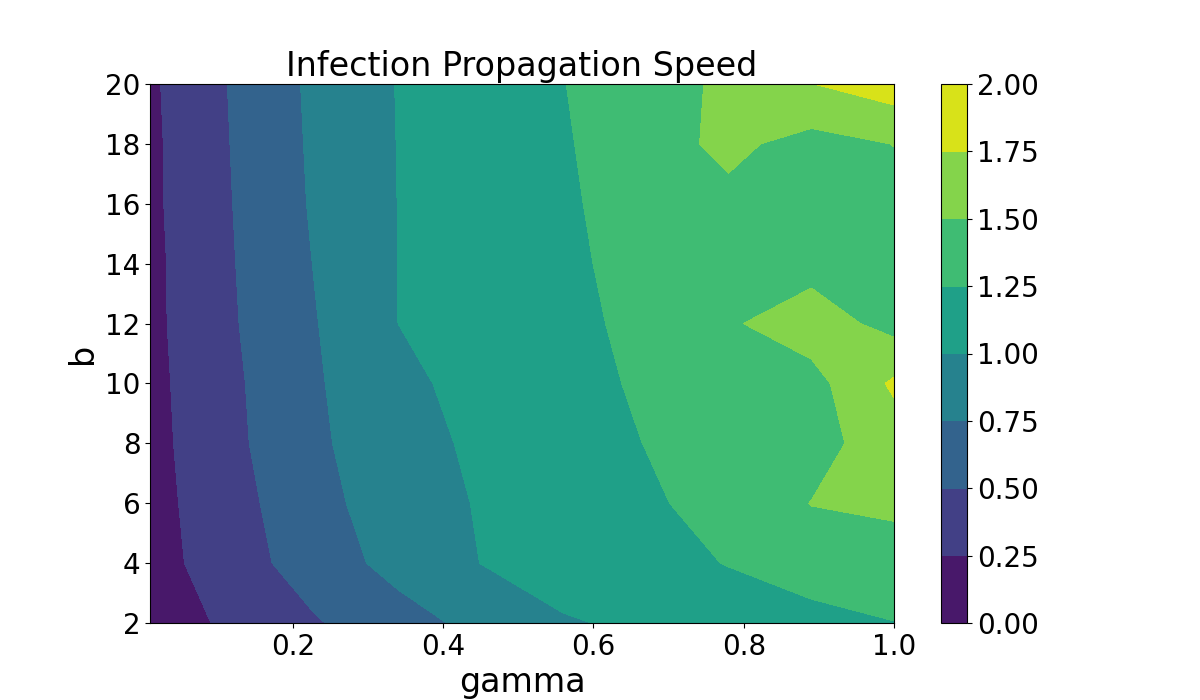
\includegraphics[scale=0.4]{./sirs_variation/infection_speed_propagation.png}
        \caption{}
        \label{fig:infection_propagation_speed}
    \end{figure}

    Examining the phase diagram, it's unsurprising that the propagation speed increases as \(\gamma\) increases. More surprisingly, it seems that the infection speed stays the same for fixed \(\gamma\) and a variety of values of \(b\). This result is not clear to us just from the equations of the PDE, and we would have expected perhaps a more complicated relationship between \(b, \gamma\) and the infection propagation speed. Additionally, there are some interesting departures from the general trend of the phase diagram for \(\gamma \approx 1\). It's not clear from the equations why this is the case, and further work should certainly investigate the \(\gamma \approx 1\) setting. In terms of policy implications, the main takeaway is that spatial infection spread is mostly modulated by the parameter \(p_i\) and so travel restrictions (reducing \(\gamma\)) are much more effective than policies aimed at reducing social distancing (reducing \(b\)).

    A limitation of this model is that people are assumed to be distributed homogenously across the grid. In reality, there are densely populated regions and sparsely populated regions. A more realistic model would incorporate this heterogenous population density and investigate how infection propagation speeds are affected. For example, one might expect the speeds to be much slower in Nebraska (predominantly rural) versus California (containing large densely populated regions). The results likely will be nuanced in the face of such heterogeneity.
    
    \newpage 

    \section{Spatial structure for discrete SIR model with 'lockdown' measure} \label{appendix:sirs_discrete}
    The spatial structure is achieved by putting the discrete model onto a 2 dimensional grid with length $L$. You can image it as a country with area $L \times L$. And one person can now only interact with the other person when he or she is within the square of length $2D_0$ whose center is that person. By tuning this new parameter $D_0$, we can now mimic the effects of 'lock down' measurement \cite{kaxiras2020multiple}.

    For example, we can make $D_0$ time-dependent \cite{kaxiras2020multiple}:
    \begin{equation}
    \label{D0}
    D_{0}(t)=\left\{ \begin{array}{lcl}
    D_0 & \mbox{for}
    & t \leq T_0  \\
    D_{0}e^{-(t - T_0)/\lambda} & \mbox{for} & t > T_0
    \end{array}\right.
    \end{equation}
    The $T_0$ represents the timing of 'lock down' while the $\lambda$ represents how fast the 'lock down' take into effect. Assuming $\lambda > 0$, as $t \to +\infty$, $D_0 \to 0$. Thus, people are being confined into a small place and cannot affect each other. By changing $T_0$ and $\lambda$ and monitoring how the three types of population evolve with time, we can then answer the questions relate to the effects of 'lock down'.
    
    Here, for simplicity, we set grid length $L = 1$ and first use the same $k, b, N, s_0, i_0$ values as Figure \ref{fig:discrete_simulation0} and explores the effects of $D_0$ when there is no 'lock down' ($T_0$ is very large). From Figure \ref{fig:d=l}, we can see when $D_0 = L$ (one person can interact with any other person on the grid), we get the same result as Figure \ref{fig:discrete_simulation0}, which is expected. From Figure \ref{fig:d=l/4} to \ref{fig:d=l/16}, the plots show that with the decrease of $D_0$, the peak of infection rate goes down and the time for reaching peak infection also delays. These results are inline with our intuition since the less the people can move and contact other people, the more difficult the disease can spread.
    
    \begin{figure}[h]
        \centering
        \begin{minipage}[b]{0.4 \textwidth}
            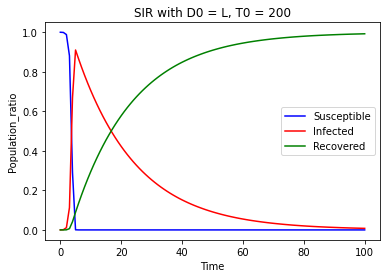
\includegraphics[width=\textwidth]{./discrete/sir_discrete_grid0.png}
            \caption{}
            \label{fig:d=l}
        \end{minipage}
        \hfill
        \begin{minipage}[b]{0.45 \textwidth}
            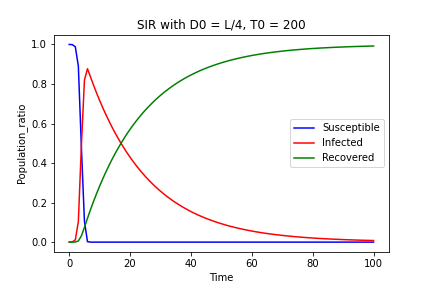
\includegraphics[width=\textwidth]{./discrete/sir_discrete_grid1.png}
            \caption{}
            \label{fig:d=l/4}
        \end{minipage}
        \centering
        \begin{minipage}[b]{0.45 \textwidth}
            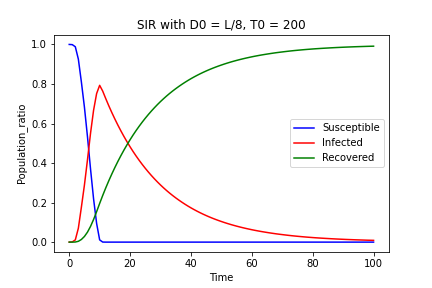
\includegraphics[width=\textwidth]{./discrete/sir_discrete_grid2.png}
            \caption{}
            \label{fig:d=l/8}
        \end{minipage}
        \hfill
        \begin{minipage}[b]{0.45 \textwidth}
            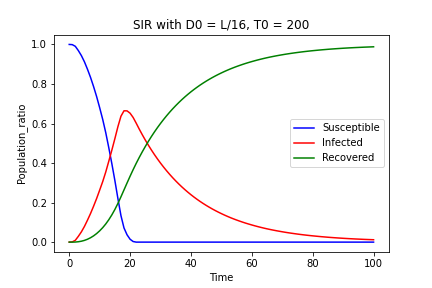
\includegraphics[width=\textwidth]{./discrete/sir_discrete_grid8.png}
            \caption{}
            \label{fig:d=l/16}
        \end{minipage}
    \end{figure}
    
    To show how the disease spreads spatially, we can visualize the grid with scatter plot of infected people. From Figure \ref{fig:day0} to \ref{fig:day5}, we can clearly see how one infected people at upper-right corner can spread the disease to people around him and eventually causes a pandemic.  
    
        \begin{figure}[h]
        \centering
        \begin{minipage}[b]{0.45 \textwidth}
            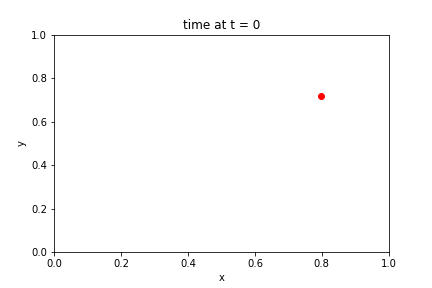
\includegraphics[width=\textwidth]{./discrete/infected_grid0.png}
            \caption{}
            \label{fig:day0}
        \end{minipage}
        \hfill
        \begin{minipage}[b]{0.45 \textwidth}
            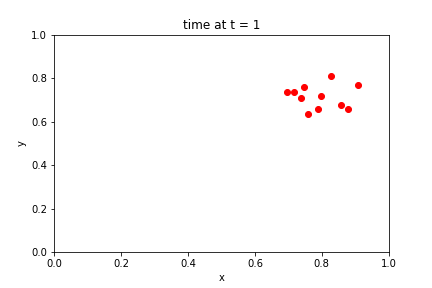
\includegraphics[width=\textwidth]{./discrete/infected_grid1.png}
            \caption{}
            \label{fig:day1}
        \end{minipage}
        \centering
        \begin{minipage}[b]{0.45 \textwidth}
            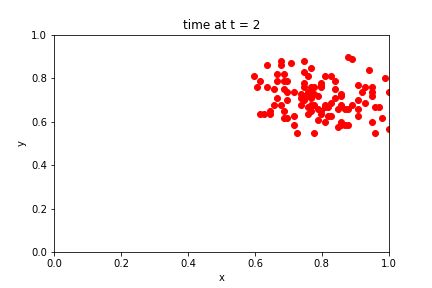
\includegraphics[width=\textwidth]{./discrete/infected_grid2.png}
            \caption{}
            \label{fig:day2}
        \end{minipage}
        \hfill
        \begin{minipage}[b]{0.45 \textwidth}
            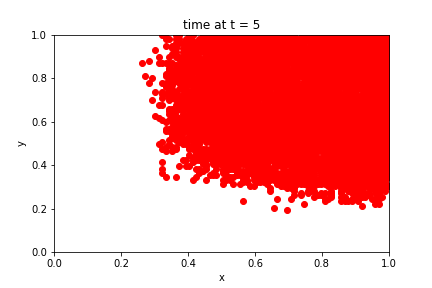
\includegraphics[width=\textwidth]{./discrete/infected_grid5.png}
            \caption{}
            \label{fig:day5}
        \end{minipage}
    \end{figure}

 \newpage 

    \section{SIR model that depends on current state} \label{appendix:sir_continous}
Figure \ref{fig:Sharp} illustrates the sharp turn as a result of concatenating systems of distinct parameters $b$ and $k$. The changes 
\begin{figure}[h]
        \centering
        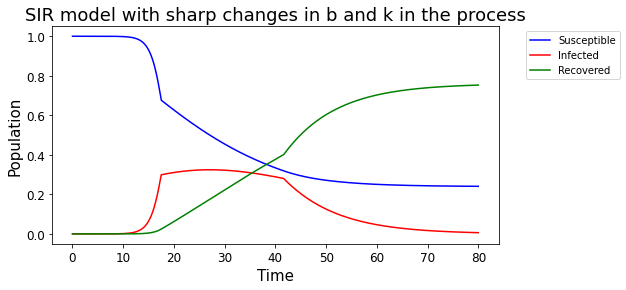
\includegraphics[scale=0.5]{./current_state_sharp_change.png}
        \caption{Sharp changes in curves  in response to changes in b and k}
        \label{fig:Sharp}
\end{figure}
In a real world setting, the values of $b$ could change multiple times depending on the current state. For instance, the government might level up the emergency response in case that the infected population continuous to grow fast and it might relax regulation when the situation becomes better. Increasing number of people are well-informed in terms of performing social distancing when more and more people get infected, but some people might start to neglect the its significance when increasing number of people get recovered. In this case, we could set up models that continuously update $b$ in response to current state such as the size of infected population. Unlike a sharp turn that is caused by an abrupt change in value of $b$ that is shown in previous discussion, the result of this continuous consideration in updating $b$ tends to smooth the curve. In the following plots, one could get an idea of how the function of $b$ could potentially impact the shape of the curve. 
\begin{figure}[h]
        \centering
        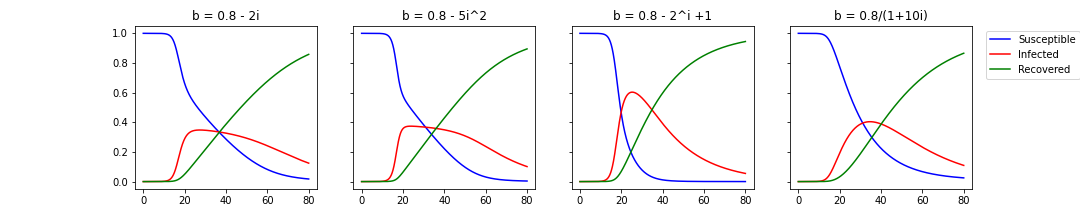
\includegraphics[scale=0.4]{./b_func.png}
        \caption{Continuously update b as a function of infected population size}
        \label{fig:cont} 
\end{figure}
Note that these functions are set in a way such that at the start of the simulation $b$ would be close to its given value. Moreover, the functions have been set to have minimum value of 0.01 in order to avoid negative $b$ values. Future analysis may adopt this consideration of changing values in $b$. One may want to use real world data and try to find the function of $b$ that makes the prediction of the model best fit the curves in real world. Together with other parameters and data, this may help to analyze in what ways do media exposure on infected population and government agencies responses gradually impact the rate of infection.


    \newpage
    \bibliographystyle{unsrt}
    \bibliography{disease}

\end{document}
